\section{Software Design Methodology}
A large focus on this group project was using an Agile development approach, similar to the Scrum iterative and incremental process (see figure 2.1 below). The idea behind Agile is to maximise the flexibility of the development process and assist in communication. Wherever possible we tried to apply these concepts to our planning and the way that we worked. The sprint system allows us to refocus our goals regularly and requires meetings to discuss progress. Excluding Sprint Zero\cite{boa}, we had three week sprints, starting on Mondays and ending on Fridays. Our Product Owner was Ed Cresswell from G-Research.  Ideally we would have liked to have shorter sprints but were limited by our product owner not being on campus. We chose to not have a Scrum Master and we used Trello\cite{trello} instead of a physical task board.

\begin{figure}[H]
\centering
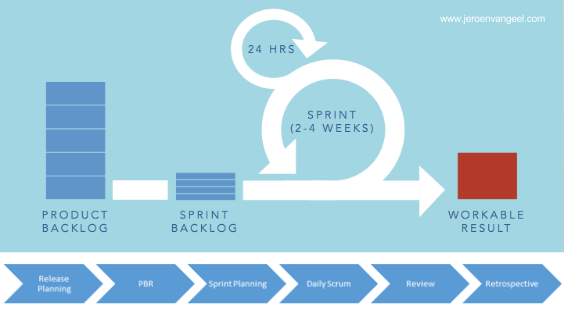
\includegraphics[scale=0.7]{sprint.png}
\caption{Scrum iterative and incremental process.}
\label{fig:scrum}
\end{figure}

Due to our Product Owner's busy schedule and the difficulty in having to travel to meet with us, we were only able to meet with him every 3 weeks for sprint reviews following sprint planning. We met on a regular basis in the college, but did not have a formal stand-up since we rarely had free time together in the labs and mainly worked at home.


\section{Risks and Issues}
Before thorough planning we considered the risks and issues that we might face during the duration of the project.
\subsection{Organisational}
There were various organisational risks that we had to manage throughout the project:
\begin{itemize}
\item A limited number of meetings with our Product Owner made it difficult for them to communicate their requirements and consequently steer our development.
\item We over and underestimated our ability to deliver on the stories we committed to in a sprint, due to inexperience working in a formalised agile environment.
\item Difficulty exposing group members to all the technologies used. This made it harder for us to fill in for one another when some team members weren't available.
\item Of course, all team members had other commitments that conflict with this project's organisation, such as coursework, exams and job/placement interviews, which limited the time we could contribute.
\end{itemize}

\subsection{Ongoing}
There were also ongoing issues which could persist after the product handover to G-Research:
\begin{itemize}
\item We are producing a product on behalf of G-Research, so there are questions relating to the final product shipping:
\begin{itemize}
\item G-Research pitched this same project to both Cambridge and Oxford.
\item G-Research want ownership of the project.
\item The project we developed had to be self-contained, it couldn't be tied to G-Research's software frameworks.
\end{itemize}
\item We ensured that the frameworks, libraries and resources we used have suitable licenses, considering that we developed the product for use in a corporate environment.
\end{itemize}

\section{Estimation of Work}
Sprint Zero was an opportunity to gauge the rate at which we worked as a group, to assist in future estimation. We swiftly developed an entire slice of our software stack - we created a basic prototype to give us an idea of the difficulty of our planned features. For example, within a few days we created a car model in Unity that met our simulation requirements (see figure 2.2 below). Off the back of this we increased our product scope to include more elaborate car physics, expecting to spend a lot of time on stretch requirements (e.g. multiple vehicle types and introducing powerups). This also influenced our thinking when estimating the size of future tasks. We expected that after Sprint Zero that physics work in Unity would take less time than we initially estimated.


\begin{figure}[H]
\centering
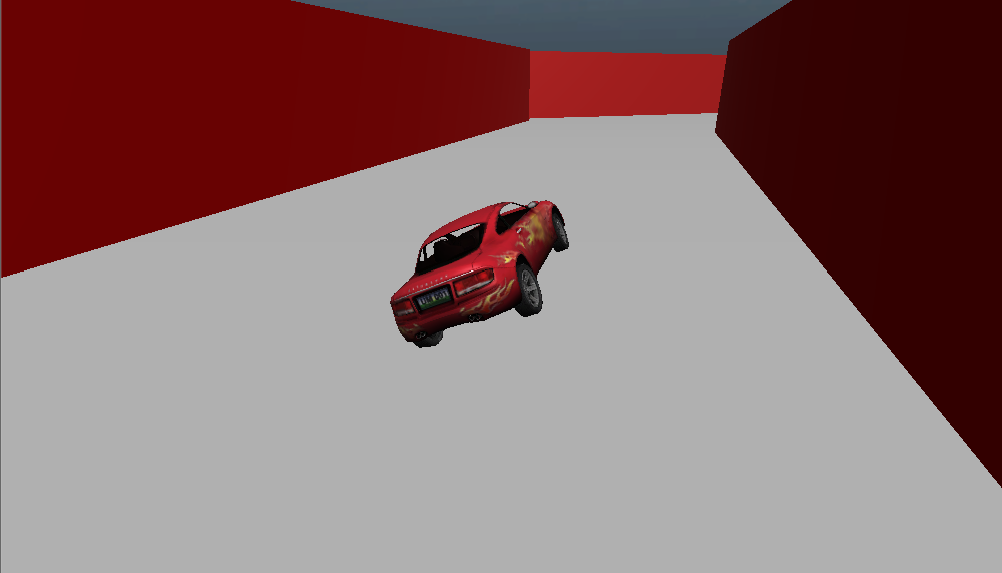
\includegraphics[scale=0.2]{prototype.png}
\caption{Early prototype}
\end{figure}

We used story points as a metric to measure the amount of effort required to implement a story. These points are displayed on each Trello card to easily differentiate major and minor tasks. As the project progressed, we compared the total story point difference between tasks planned and tasks completed in each sprint. This indicated whether we under or overestimated our workload during sprint planning. As we have worked in numerous group projects together, we already had a rough baseline in our minds for estimating task size. We used this notion when assigning story points to tasks in our backlog.

\section{Creating a Plan}
The first day of our project began with a struggle - a serious lack of direction. We were given a short paragraph describing our task, and unfortunately that was all the instruction we had for two weeks of work. While most groups met with their supervisors within the first few days, our product owner was hard to reach as we couldn't contact him directly (Our group $\rightarrow$ Marc, Imperial contact $\rightarrow$ Emily, G-Research HR $\rightarrow$ Ed, G-Research product owner). Due to the difficulty in communicating with our product owner, we were unable to setup an initial planning meeting until close to our first deadline.  In fact, for our first week we were unsure if the meeting would occur at all.

So we were faced with a hard decision, should we hold off on development until we could form a plan with Ed, or carry on undirected? It was clear that both options had risks, if we coded our own vision it could be rejected by our client and result in a huge waste of our time. And yet, if we were to stall for that initial meeting we might have to keep pushing back our work until it was deadline night, whereby our work would be reviewed the next morning! Ultimately we chose to charge on unaided, believing some progress is better than none, which strongly influenced the evolution of our plan. 

A key component to the success of a group lies within its ability to stay self motivated. With the looming threat of our work being scrapped when our first meeting arrived, we delegated work by interest. Ensuring that everyone was coding parts they were excited to be coding allowed us to justify working hard even if the project went in the wrong direction and had to be scaled back.

Clients are well known for their sudden changes in requirements and wishes (and we hadn't even met this client yet) so our plan had to be flexible enough to handle just about anything. To maintain this flexibility we frequently discussed our progress, trying to place ourselves in G-Research's shoes and imagining what they would want us to achieve. Wherever possible we focused on work that had to be done regardless of a change in requirements. Tasks such as setting up the VM, installing development tools, and learning about technologies directly specified in the project description - such as Unity.

We began Sprint Zero with a short sighted approach to planning, focusing on what we could achieve today rather than working toward a long time goal. While this made sense before meeting our PO Ed, afterwards we had more of G-Research's goals in mind, specifically that we were designing our project to be used at a career fair. With this new insight we refocused our direction and aimed to simplify our API. This was one of the few changes we had to make after first meeting Ed, highlighting how successful we were in producing code unlikely to change in the face of changing requirements. Establishing the initial contact with Ed and being able to discuss what to focus our efforts on for each split made subsequent Sprints far simpler to plan.

\section{Tracking Progress and Managing Work}

\subsection{Agile}
To track our progress on this project we maintained a Product Backlog and Sprint Backlog. Our Product Backlog lists all of the features that the client requires in the final product, as well as some possible extensions. The Sprint Backlog tracks items that should be completed within the current three week sprint, and are filled from the Product Backlog. The features with the highest priority in the Product Backlog were chosen first - these may be broken down into smaller tasks if a major feature cannot be implemented in one sprint cycle. Splitting up larger features also made it easier to estimate the size of the tasks as well as making progress easier to track. As the Product Backlog was filled, individuals or pairs were assigned to tasks until all group members had a clear understanding of what they need to accomplish over the coming three weeks. Being able to see what individuals were working on at a glance ensured that no-one stepped on each others toes when developing.

Along with the Sprint Backlog, we maintained a Doing and Done list for tasks in a sprint. This allowed us to check our progress of the current sprint by glancing at which columns the tasks were in. We used this to adapt our work according to our other varying commitments and how fast we completed the tasks we were focusing on at the time - when sprint tasks were being completed early we were able to add additional tasks partway throughout the sprint.

Beyond managing our work, we needed to be adaptable - as listed in our plan, there were many organisational risks and issues which could affect the team's performance (e.g. inflexible roles) that we had to be mindful of. Having Sprint Retrospectives immediately after each Sprint Review allowed us to evaluate and improve our development process so subsequent sprints could flow better. This was also a key moment where all group members could get together and discuss the current status of the project, considering that we all had various conflicts that led to our work times being disjointed. Any issues or improvements raised would then be added to Trello for the following sprint.

\subsection{Trello}
We used Trello as a task board, creating cards for stories and checklists for tasks. Using the `Scrum for Trello' Chrome plugin\cite{scrumfortrello}, we were able to assign story points to each card and visualise progression on a burndown chart. We decided to use one board as opposed to a new one for each sprint for ease of maintenance and monitoring progression against the product backlog. We made use of labels to denote cards that are blocked, introduced late in a sprint (i.e. after planning) or not finished during a previous sprint. This proved to be useful during retrospectives when assessing how effective our planning was.

\subsection{Facebook Chat}
We also had a Facebook chat for our project, for simple communicating when working in a distributed manner. While Facebook chat is a fairly simple tool, it was especially useful for deciding when we want to meet up, or for quick discussions about project progress (e.g. bugs and other blockers).

\subsection{git}
As with all our project work at Imperial, we used git for our version control, hosting on our private Github repository. This worked well for group organisation and eases the handoff to G-Research, as they can clone our repository and be almost ready to go. Our use of branches over the course of the project worked well with our Agile development methodology, as each story in our Sprint could be handled on a seperate branch. This allowed stories to be focused on in isolation. Additionally, any group member interested in the progress of a story can simply read the git logs for a branch and be up to speed with no clutter from other stories in development.

\iffalse
Since we using git for our version control, and Github as our host for the project, we made use of Github's in-built issue tracking system. (Currently we use Trello to flag up issues, sometimes breaking our task board story-system by making a new card just for the issue. Using a dedicated system could help organise what problems we are having, in particular which issues are preventing further work from being completed. However, Github's 'Issues' feature isn't just restricted to bug fixes; it can be used for enhancements and keeping track of who is working on what, so it might be worth using this as an alternative, or in addition to Trello.) (Did we even use this?)
\fi

\section{Team Roles}
\subsubsection{Christophe}
Worked in Unity on the car simulation, designed and implemented the Unity HUD and race victory conditions. Christophe also created the effects such as skidmarks, sound and field of view changes when boosting.

\subsubsection{Finlay}
Finlay worked predominantly on the Unity side of the project. He worked on designing and implementing the AI API, including the lane based spline following system and the system needed for providing corner information. He also constructed racetracks using tools and assets from the Unity Asset Store along with adding new scripts for tasks such as managing cars and starting races.

\subsubsection{Louis}
Louis worked on the browser front-end, helping with the design and tasks such as setting up the authentication system. He also worked on communication between the Unity web player and the website, allowing Unity to send metrics to the database which he then used to create the leaderboard and ranking system.

\subsubsection{Ben}
Ben primarily dealt with the back-end, implementing Node.js and MongoDB. He setup TeamCity, allowing automatic deployment and multiple live builds.  On the front-end, he migrated the script execution from Unity to the browser - allowing user to write JavaScript. Furthermore, he built the browser's tournament and live editing features. Finally, he designed and created the Event API and CoffeeScript extensions.

\subsubsection{Jaime}
On the Unity side, Jaime designed additional tracks, as well as implementing the car colours, car model selector and enabling the boost function. He also worked on the front-end, implementing administrator functionality.  


\subsubsection{Thomas}
Thomas worked on the browser front-end, both designing and implementing the website, including integration of the Ace editor. He created the instructional handout and held the collaborative user testing (described in the Evaluation chapter).
